\documentclass{report}
\usepackage{pdfpages}
\usepackage{graphicx} 
\usepackage{dirtytalk}
\usepackage{lmodern}
\usepackage{booktabs}
\usepackage{listings}
\usepackage{float}
\usepackage{siunitx}
\usepackage{amsmath}
\usepackage{rotating}
\usepackage{arydshln}
\usepackage[hidelinks]{hyperref}
\usepackage[ngerman]{babel}
\usepackage[a4paper, total={6in, 8in}]{geometry}
\begin{document}
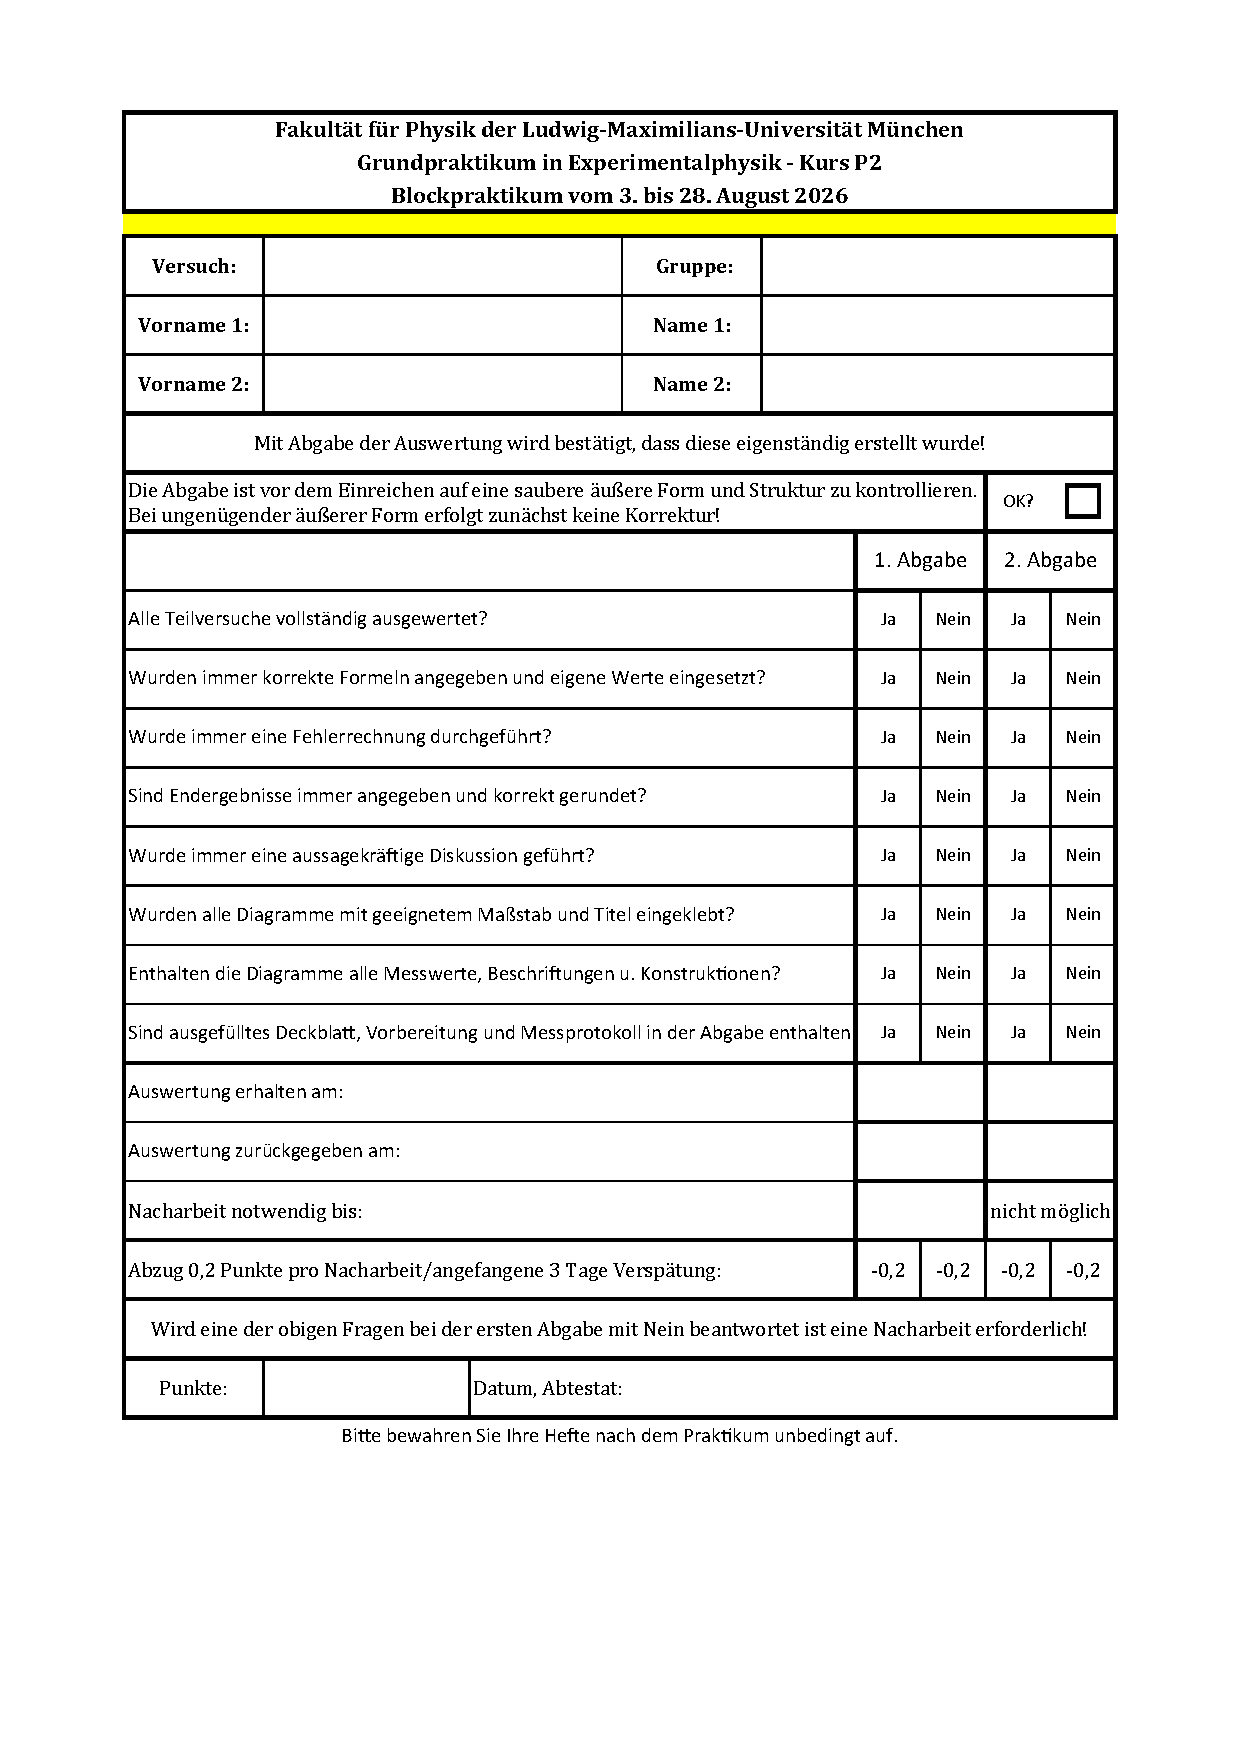
\includepdf[pages=-]{./PDFs/Deckblatt_P2.pdf}
\begin{titlepage}
    \begin{center}
        \vspace*{1cm}
            
        \Huge
        \textbf{Auswertung und Protokoll}
            
        \vspace{0.5cm}
        \LARGE
        Zum Versuch OSZ
        
        \vspace{1.8cm}

        \textbf{Jonas Müther \& Alejandro Schultheiss}
        \vfill
            
        P2 Praktikum\\
       
            
        \vspace{0.8cm}
  

        \vspace{1.8cm}
        \Large
        LMU München \\
        Physik B.Sc.\\
        Deutschland\\
        2026
            
    \end{center}
\end{titlepage}
\tableofcontents

\newpage
\chapter{Vorbereitung}

\section{Versuchsvorbereitung und Grundlagen des Versuchs}
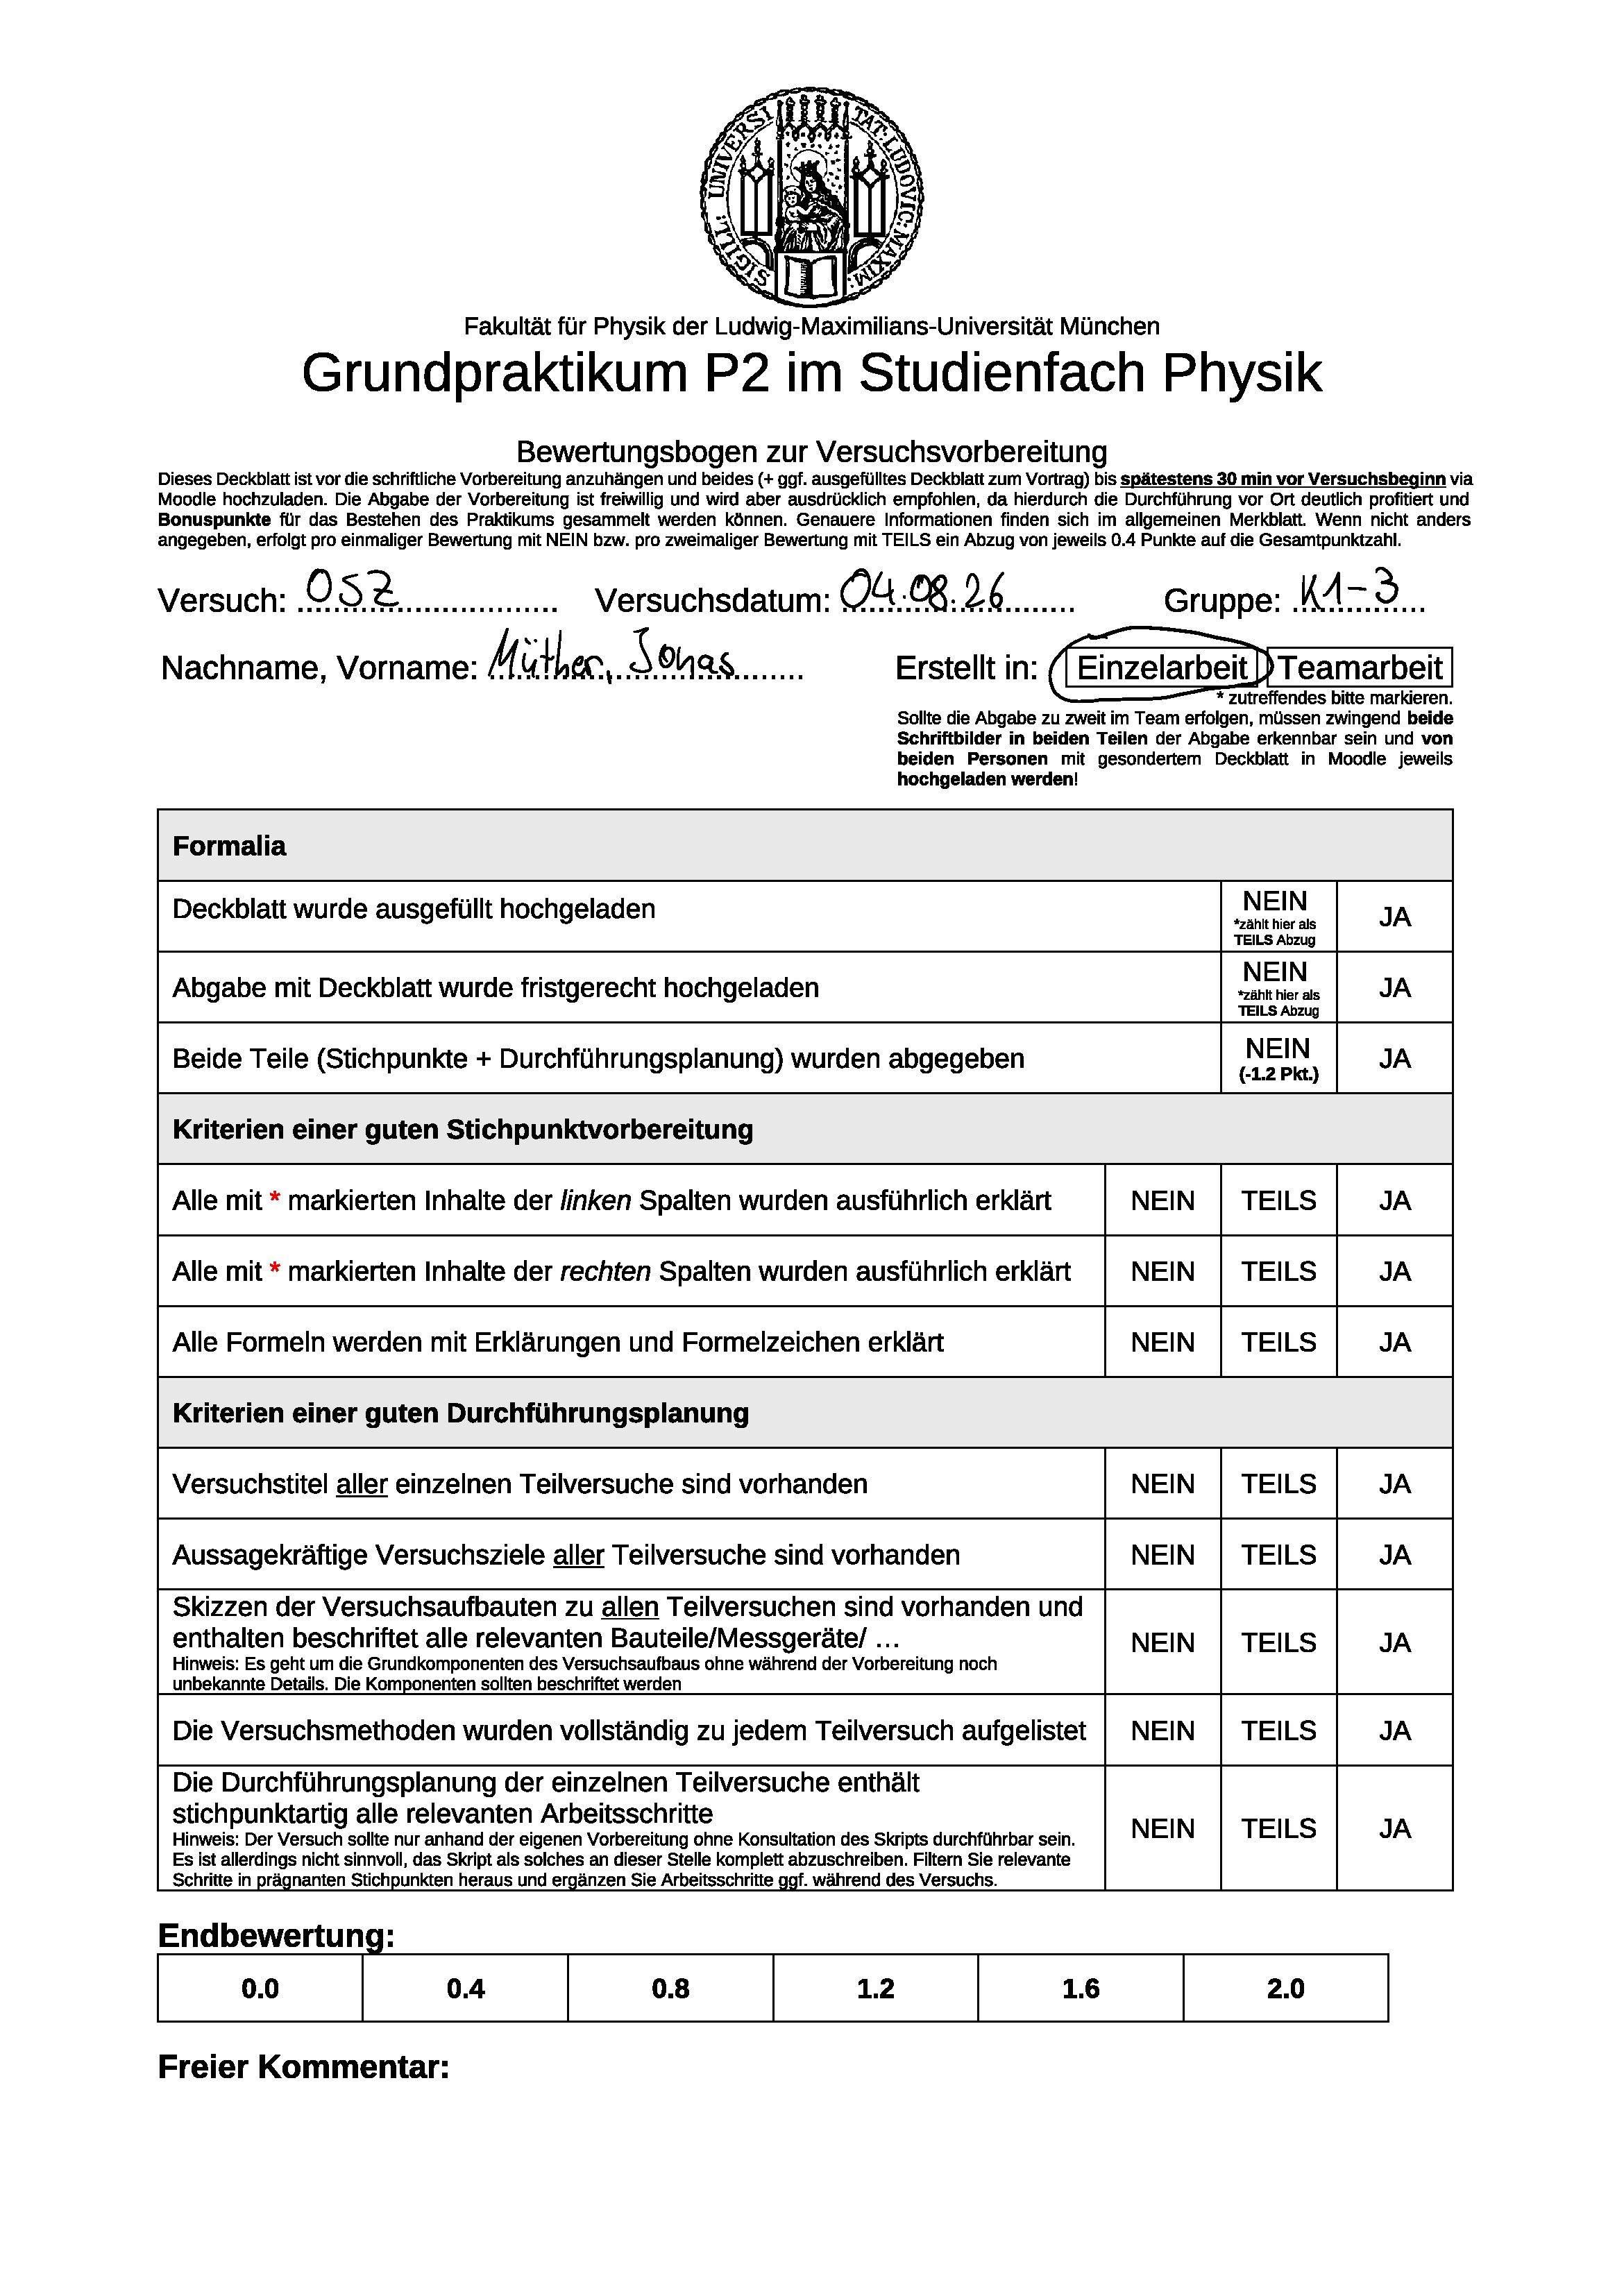
\includepdf[pages=-]{./PDFs/VorbereitungOSZ.pdf}

\section{Versuchsprotokoll}
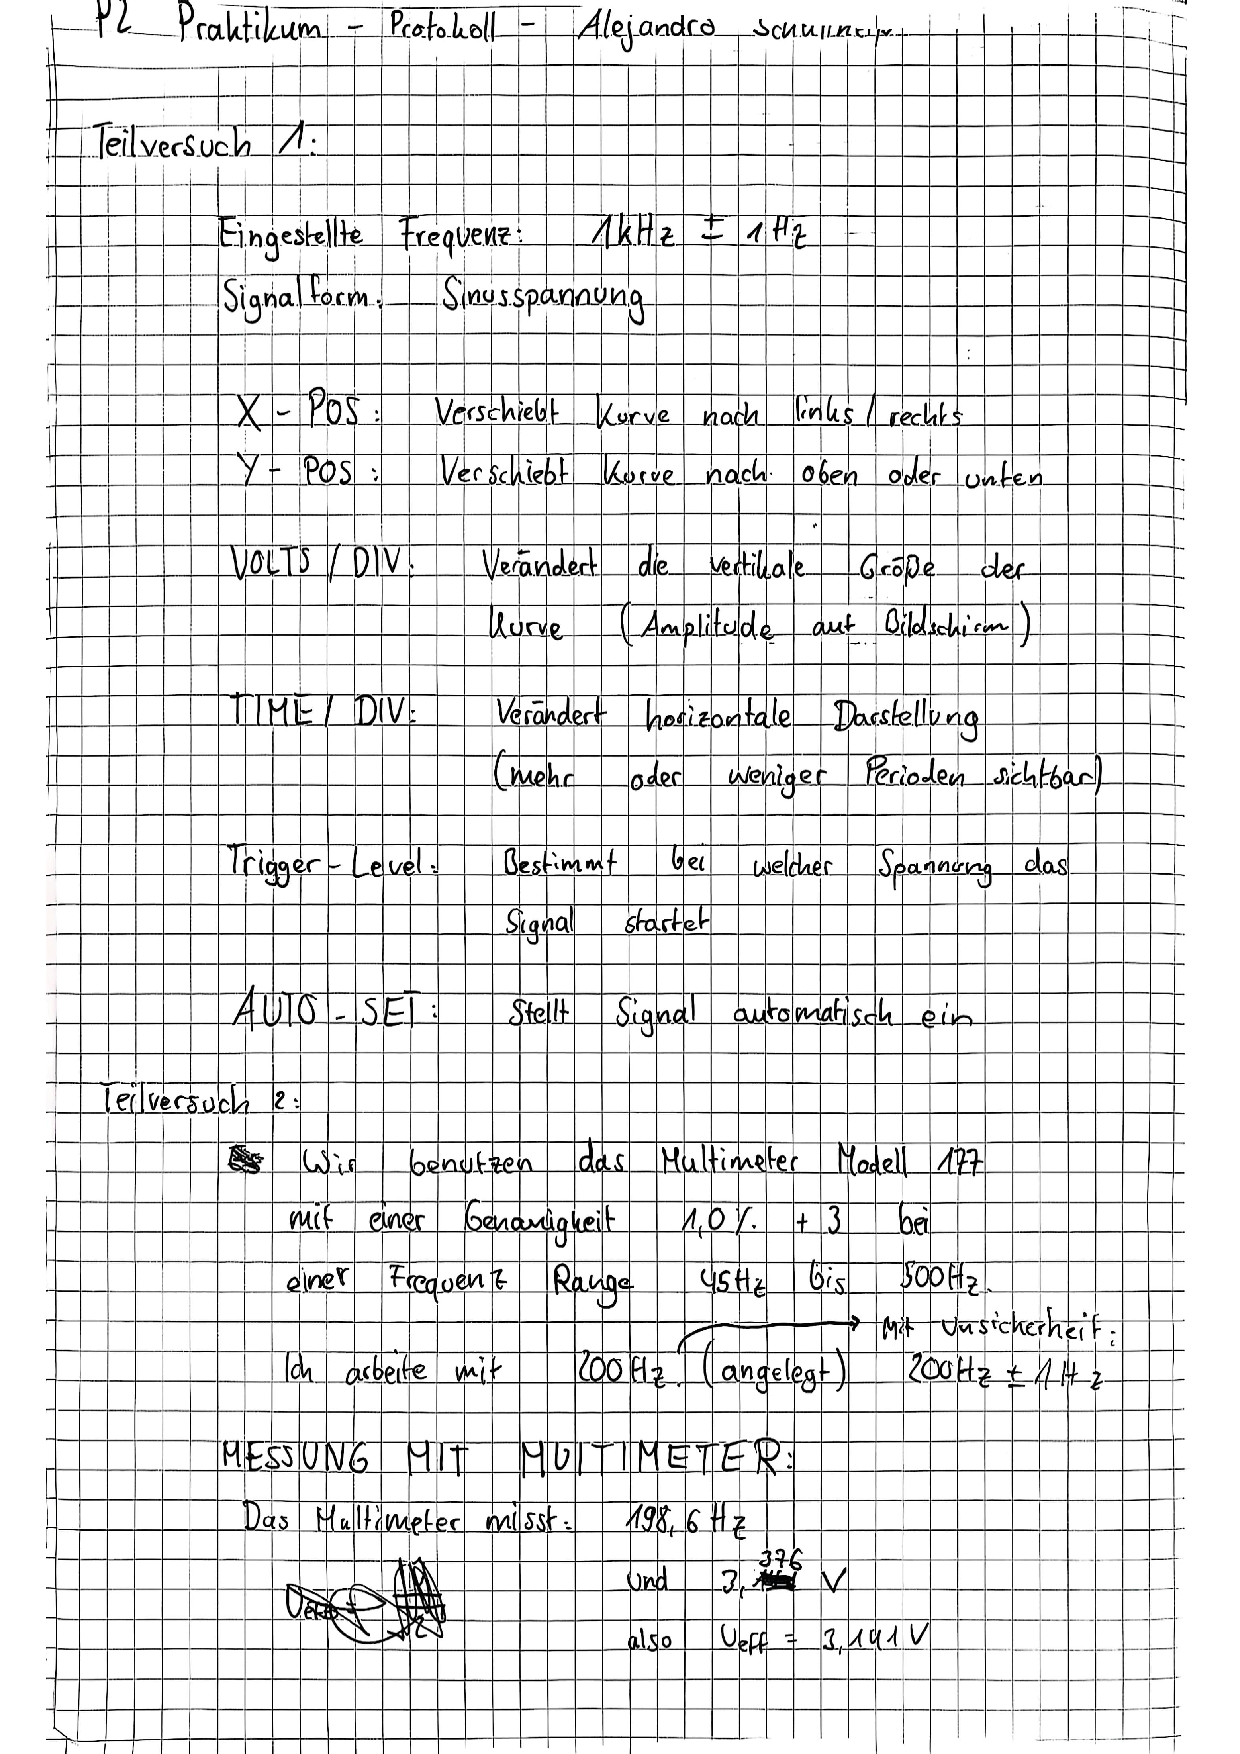
\includepdf[pages=-]{./PDFs/OSZProtokoll.pdf}

\newpage
\chapter{Auswertung}
\section{Teilversuch I: Basisbedienelemente eines Oszilloskops}
Dieser Teilversuch diente dazu, sich mit den Basisbedienelementen eines Oszilloskops vertraut zu machen.
\subsection{Positionseinstellungen}
Ein Oszilloskop hat eine x- und y-Positionseinstellung. Mit der x-Einstellung kann die Position des gemessenen 
Signals auf dem Bildschirm in Horizontaler Richtung verschoben werden. Mithilfe der y-Einstellung kann das Signal in vertikale
Richtung verschoben werden. Hierzu wird jeweils ein Drehknopf verwendet.
\subsection{Ablenkfaktoren}
Mit den Ablenkfaktoren kann die Skalierung des Signals in x- und y-Richtung auf dem Bildschirm angepasst werden. Hierzu wird
wieder ein Drehknopf verwendet. Drehen dieses Drehknopfes im Uhrzeigersinn streckt das Signal in die jeweilige Richtung. 
Der Ablenkfaktor in x-Richtung ist oft die Zeitablenkung.
Die aktuellen Werte dieser Einstellungen sind oft am Rand des Displays angezeigt. In der regel wird hier die Spannung pro Kästchen
bzw. die Zeit pro Kästchen angezeigt.
\subsection{Trigger}
Der Trigger dient dazu, den Zeitpunkt festzulegen, ab dem das Oszilloskop wieder an den linken Rand springt und dort wieder 
mit dem \glqq Zeichnen \grqq des Signals zu beginnen. Hierzu werden sowohl eine Schwelle als auch das Vorzeichen der Ableitung (Flanke)
an der Stelle des Signals angegeben, an der dieser Sprung geschehen soll. Mit einem Drehknopf verstellt man diese Spannungsschwelle. 
Mit einem Tastschalter kann dann noch eingestellt werden, ob der Sprung geschehen soll, wenn die Spannung die Schwelle 
Fallend oder Steigend durchschreitet.
Dies ist insbesondere nützlich, um bei periodischen Signalen ein stehendes Bild zu erhalten. Außerdem kann der Trigger genutzt 
werden um den Start einer gespeicherten Messung auszulösen. 

\newpage
\section{Teilversuch II: Messen einer Amplitude}
In Teilversuch II sollten die effektive Spannung einer Wechselspannung mit der Amplitude dieser verglichen werden. 
Hierzu wurde ein Funktionsgenerator mit einem Sinus-Signal an ein Oszilloskop und an ein Multimeter angeschlossen.
Hierbei wurde beobachtet, dass die am Multimeter gemessene Spannung signifikant unterhalb der Amplitude der Wechselspannung 
liegt.
\subsection{Theoretischer Hintergrund}
Der Unterschied zwischen den gemessenen Spannungen liegt daran, dass ein Multimeter die effektive Spannung misst, also den Wert, 
den eine Gleichspannung mit gleicher mittlerer Leistung hätte. Es gilt also:
\begin{equation}
    \bar{P} = \frac{U_\mathrm{eff}^2}{R} = \frac{1}{T}\int_{0}^{T} \frac{(U(t))^2}{R} \,\mathrm{d}t = \frac{1}{T}\int_{0}^{T} \frac{\hat{U}^2}{R}\sin^2(\omega t) \,\mathrm{d}t 
\end{equation}
Dies lässt sich folgenermaßen umformen:
\begin{equation}
    \begin{split}
        \frac{U_\mathrm{eff}^2}{R}          &= \frac{1}{T}\int_{0}^{T} \frac{\hat{U}^2}{R}\sin^2(\omega t) \,\mathrm{d}t \\
        \Leftrightarrow U_\mathrm{eff}^2    &= \hat{U}^2 \int_{0}^{2\pi} \frac{\sin^2(x)}{2\pi} \, \mathrm{d}x \\
        \Leftrightarrow U_\mathrm{eff}^2    &= \frac{\hat{U}^2}{2} \\
        \Leftrightarrow U_\mathrm{eff}      &= \frac{\hat{U}}{\sqrt{2}}
    \end{split}
\end{equation}
Die Unsicherheit ist gegeben durch:
\begin{equation}
    \begin{split}
        \Delta U_\mathrm{eff}    &= \frac{\partial U_\mathrm{eff}}{\partial \hat{U}} \cdot \Delta \hat{U} \\
                        &= \frac{\Delta \hat{U}}{\sqrt{2}}
    \end{split}
\end{equation}
\subsection{Auswertung der Messwerte}
In zwei Versuchsdurchgängen wurden folgende Werte für Amplitude und Effektivspannung gemessen:
\begin{table}[H]
    \centering    
    \label{tab:AmpUeff}
    \begin{tabular}{c || c | c}
        Messdurchgang  & Amplitude $(\hat{U})$ & Effektivspannung ($U_\mathrm{eff}$) \\
        \hline
        1 & $(4.89 \pm 0.10) \si{V}$ & $(3.38 \pm 0.04) \si{V}$\\
        2 & $(11.90 \pm 0.20) \si{V}$ & $(8.48 \pm 0.09) \si{V}$ \\
    \end{tabular}
    \caption{Gemessene Amplitude und Effektivspannung}
\end{table}
\noindent
Aus den gemessenen Amplituden ergeben sich damit aus der Theorie folgende effektiven Spannungen:
\begin{equation}
    \begin{split}
        U_{\mathrm{eff, 1}} = 3.46 \pm 0.08 \si{V} \\
        U_{\mathrm{eff, 2}} = 8.41 \pm 0.15 \si{V}
    \end{split}
\end{equation}
Die Werte stimmen also im Rahmen der Unsicherheiten mit den via Multimeter gemessenen effektiven Spannungen überein.

\newpage
\section{Teilversuch III: }

\newpage
\section{Teilversuch IV: }

\newpage
\section{Teilversuch V: Quantitative Registrierung der Entladekurve eines Kondensators}
In Teilversuch V sollte die Entladekurve eines Kondensators quantitativ bestimmt werden. Hierzu wurden bei zwei unterschiedlichen 
Tastkopfeinstellungen (1x und 10x) die die Entladekurven aufgezeichnet und mehrere Messpunkte aufgenommen. 
\subsection{Gemessene Daten}
\subsubsection{1x Tastkopf}
\begin{table}[H]
    \centering
    \label{tab:1xTK}
    \begin{tabular}{c | c}
        Zeit in \si{s} & Spannung in \si{V} \\
        \hline
        0.000 & 5.55 \\
        0.200 & 3.55 \\
        0.400 & 2.28 \\
        0.600 & 1.50 \\
        0.800 & 0.95 \\
        1.000 & 0.62 \\
        1.200 & 0.29 \\
        1.400 & 0.20
    \end{tabular}
    \caption{Gemessener Spannungsverlauf mit dem 1x Tastkopf}
\end{table}
Die Messunsicherheiten sind hierbei jeweils gegeben durch:
\begin{equation}
    \begin{split}
        \Delta t &= 0.01s \\
        \Delta U &= 0.05V
    \end{split}
    \nonumber
\end{equation}
\subsubsection{10x Tastkopf}
\begin{table}[H]
    \centering
    \label{tab:10xTK}
    \begin{tabular}{c | c}
        Zeit in \si{s} & Spannung in \si{V} \\
        \hline
        0.000 & 0.633 \\
        0.200 & 0.500 \\
        0.400 & 0.388 \\
        0.600 & 0.309 \\
        0.800 & 0.241 \\
        1.000 & 0.190 \\
        1.200 & 0.250 \\
        1.400 & 0.120 \\
        1.600 & 0.093
    \end{tabular}
    \caption{Gemessener Spannungsverlauf mit dem 1x Tastkopf}
\end{table}
\begin{equation}
    \begin{split}
        \Delta t &= 0.01s \\
        \Delta U &= 0.005V
    \end{split}
    \nonumber
\end{equation}
\newpage
Aus diesen Werten ergeben sich folgende Diagramme:
\begin{figure}[H]
    \centering
    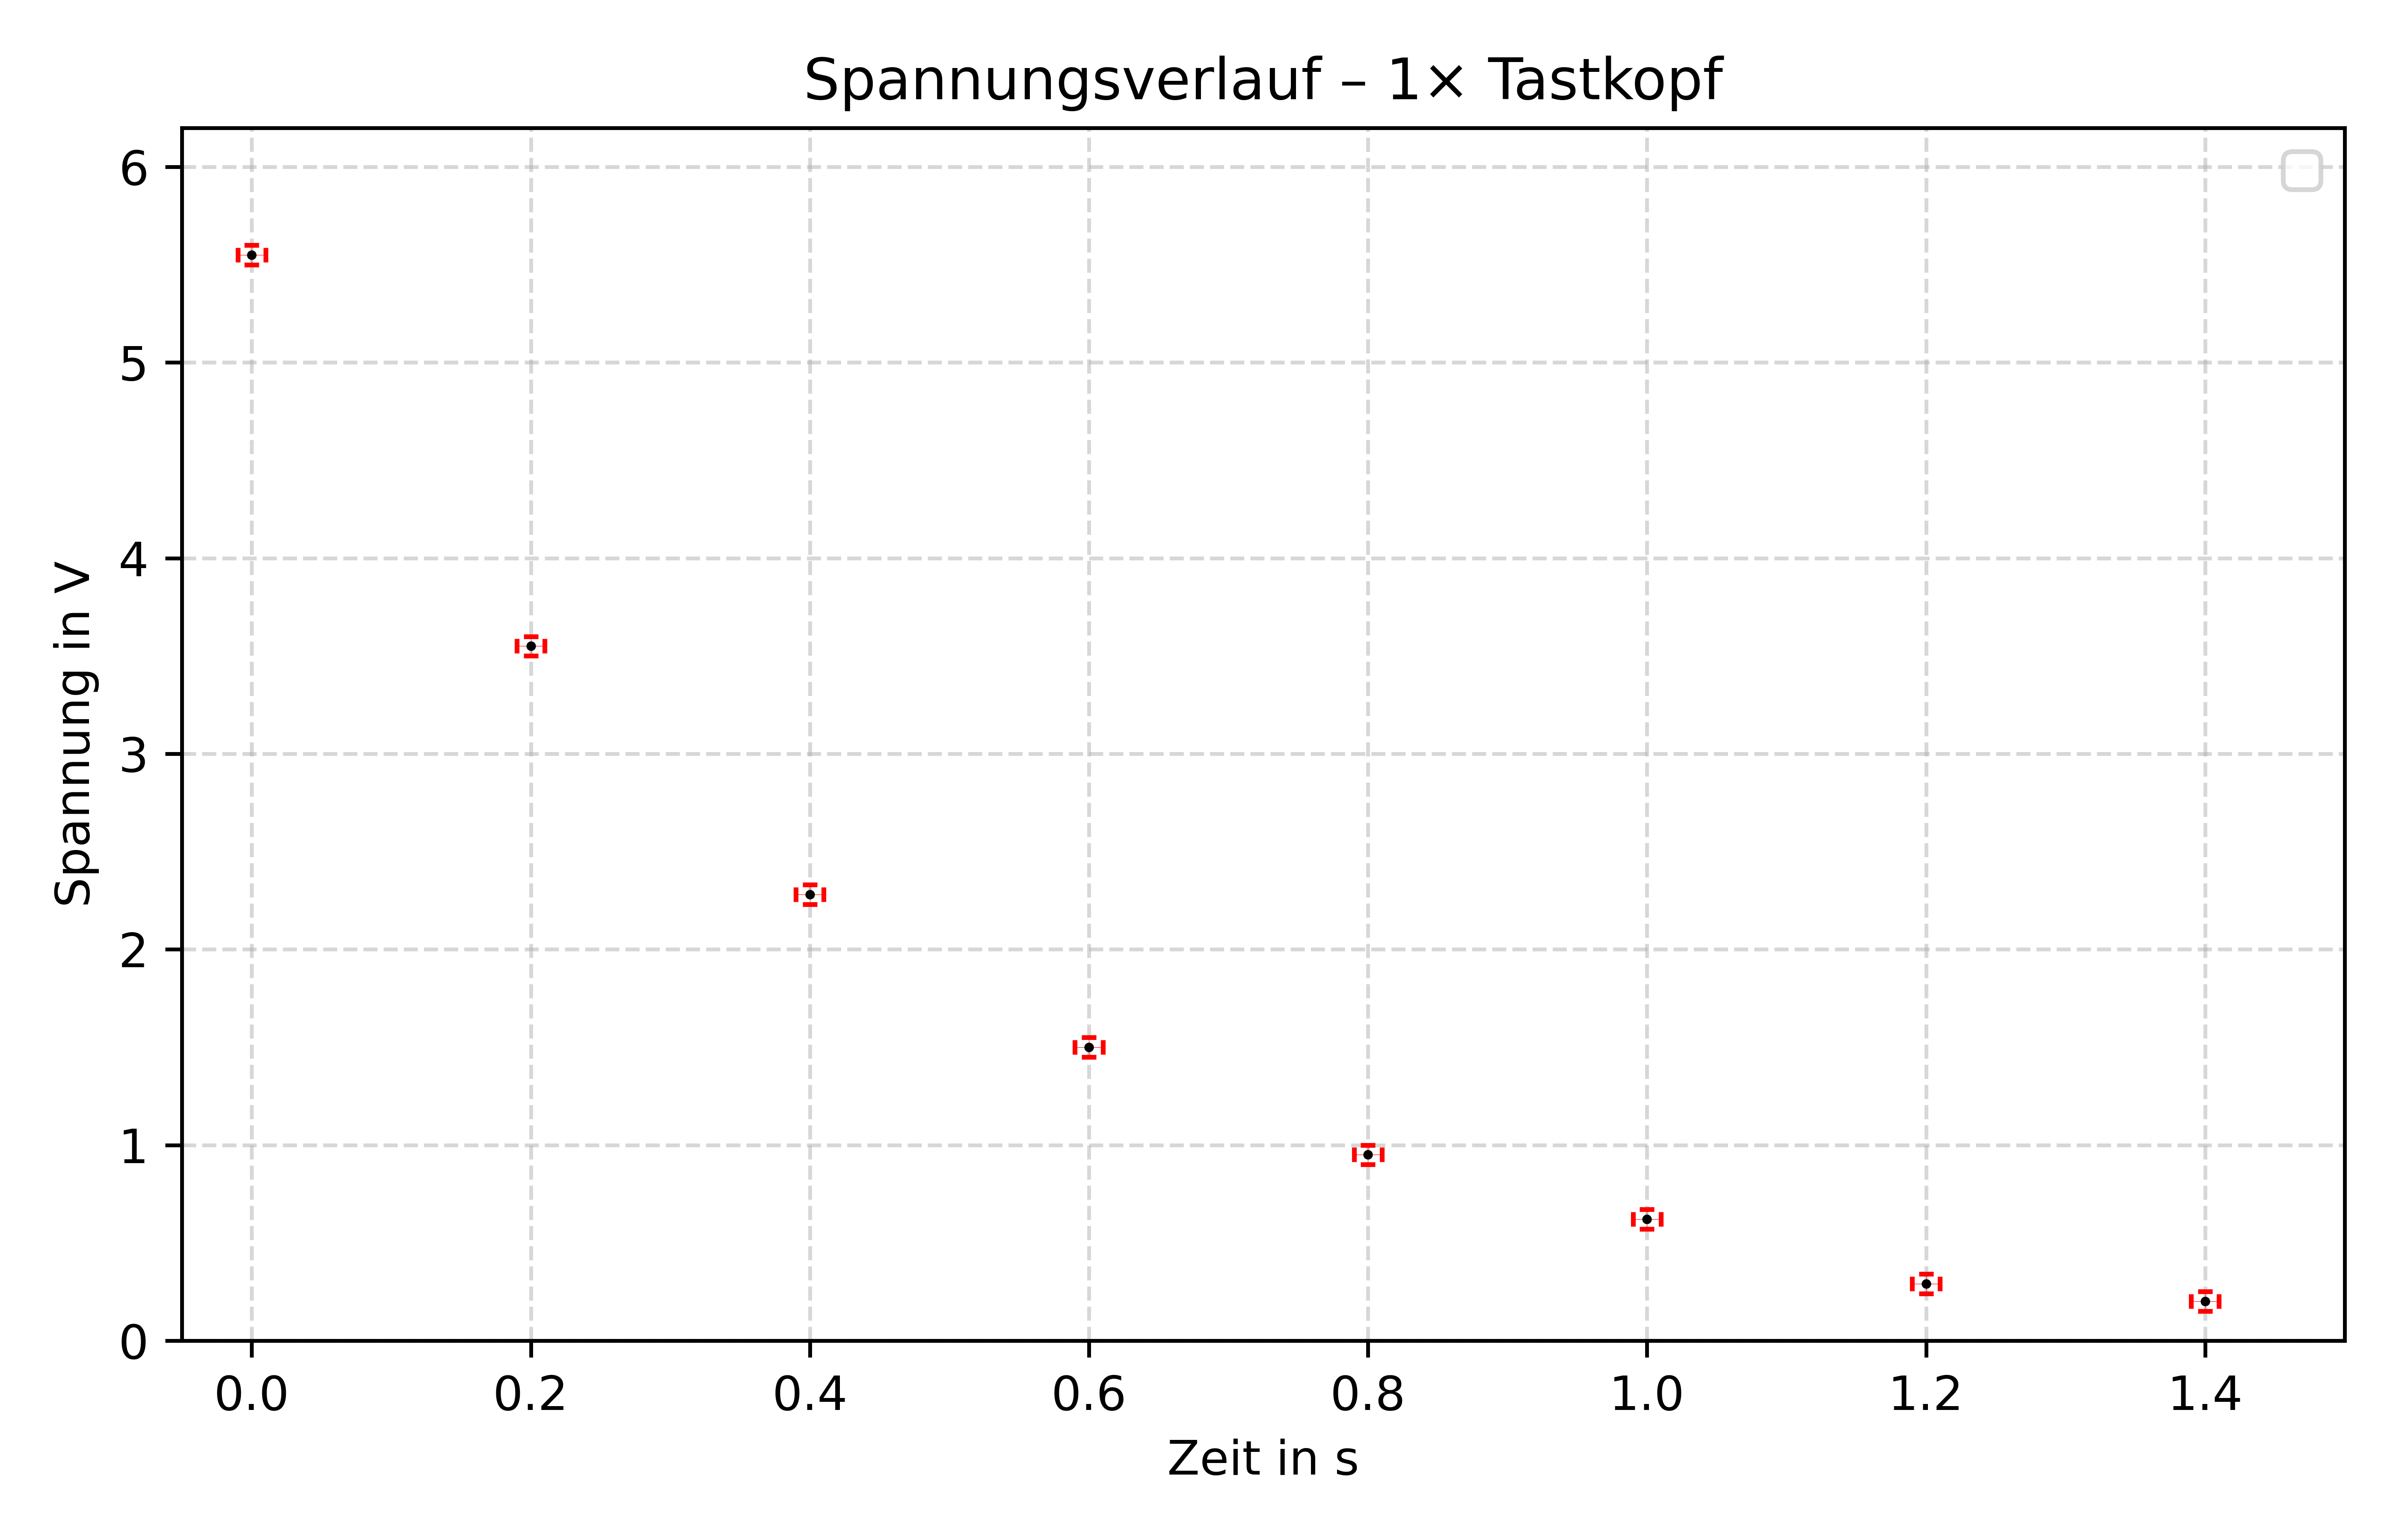
\includegraphics[width=.8\textwidth]{./Images/spannungsverlauf_1xTKRaw.png}
    \caption{Spannungsverlauf 1$\times$ Tastkopf}
    \label{fig:1xTKDiag}
\end{figure}
\begin{figure}[H]
    \centering
    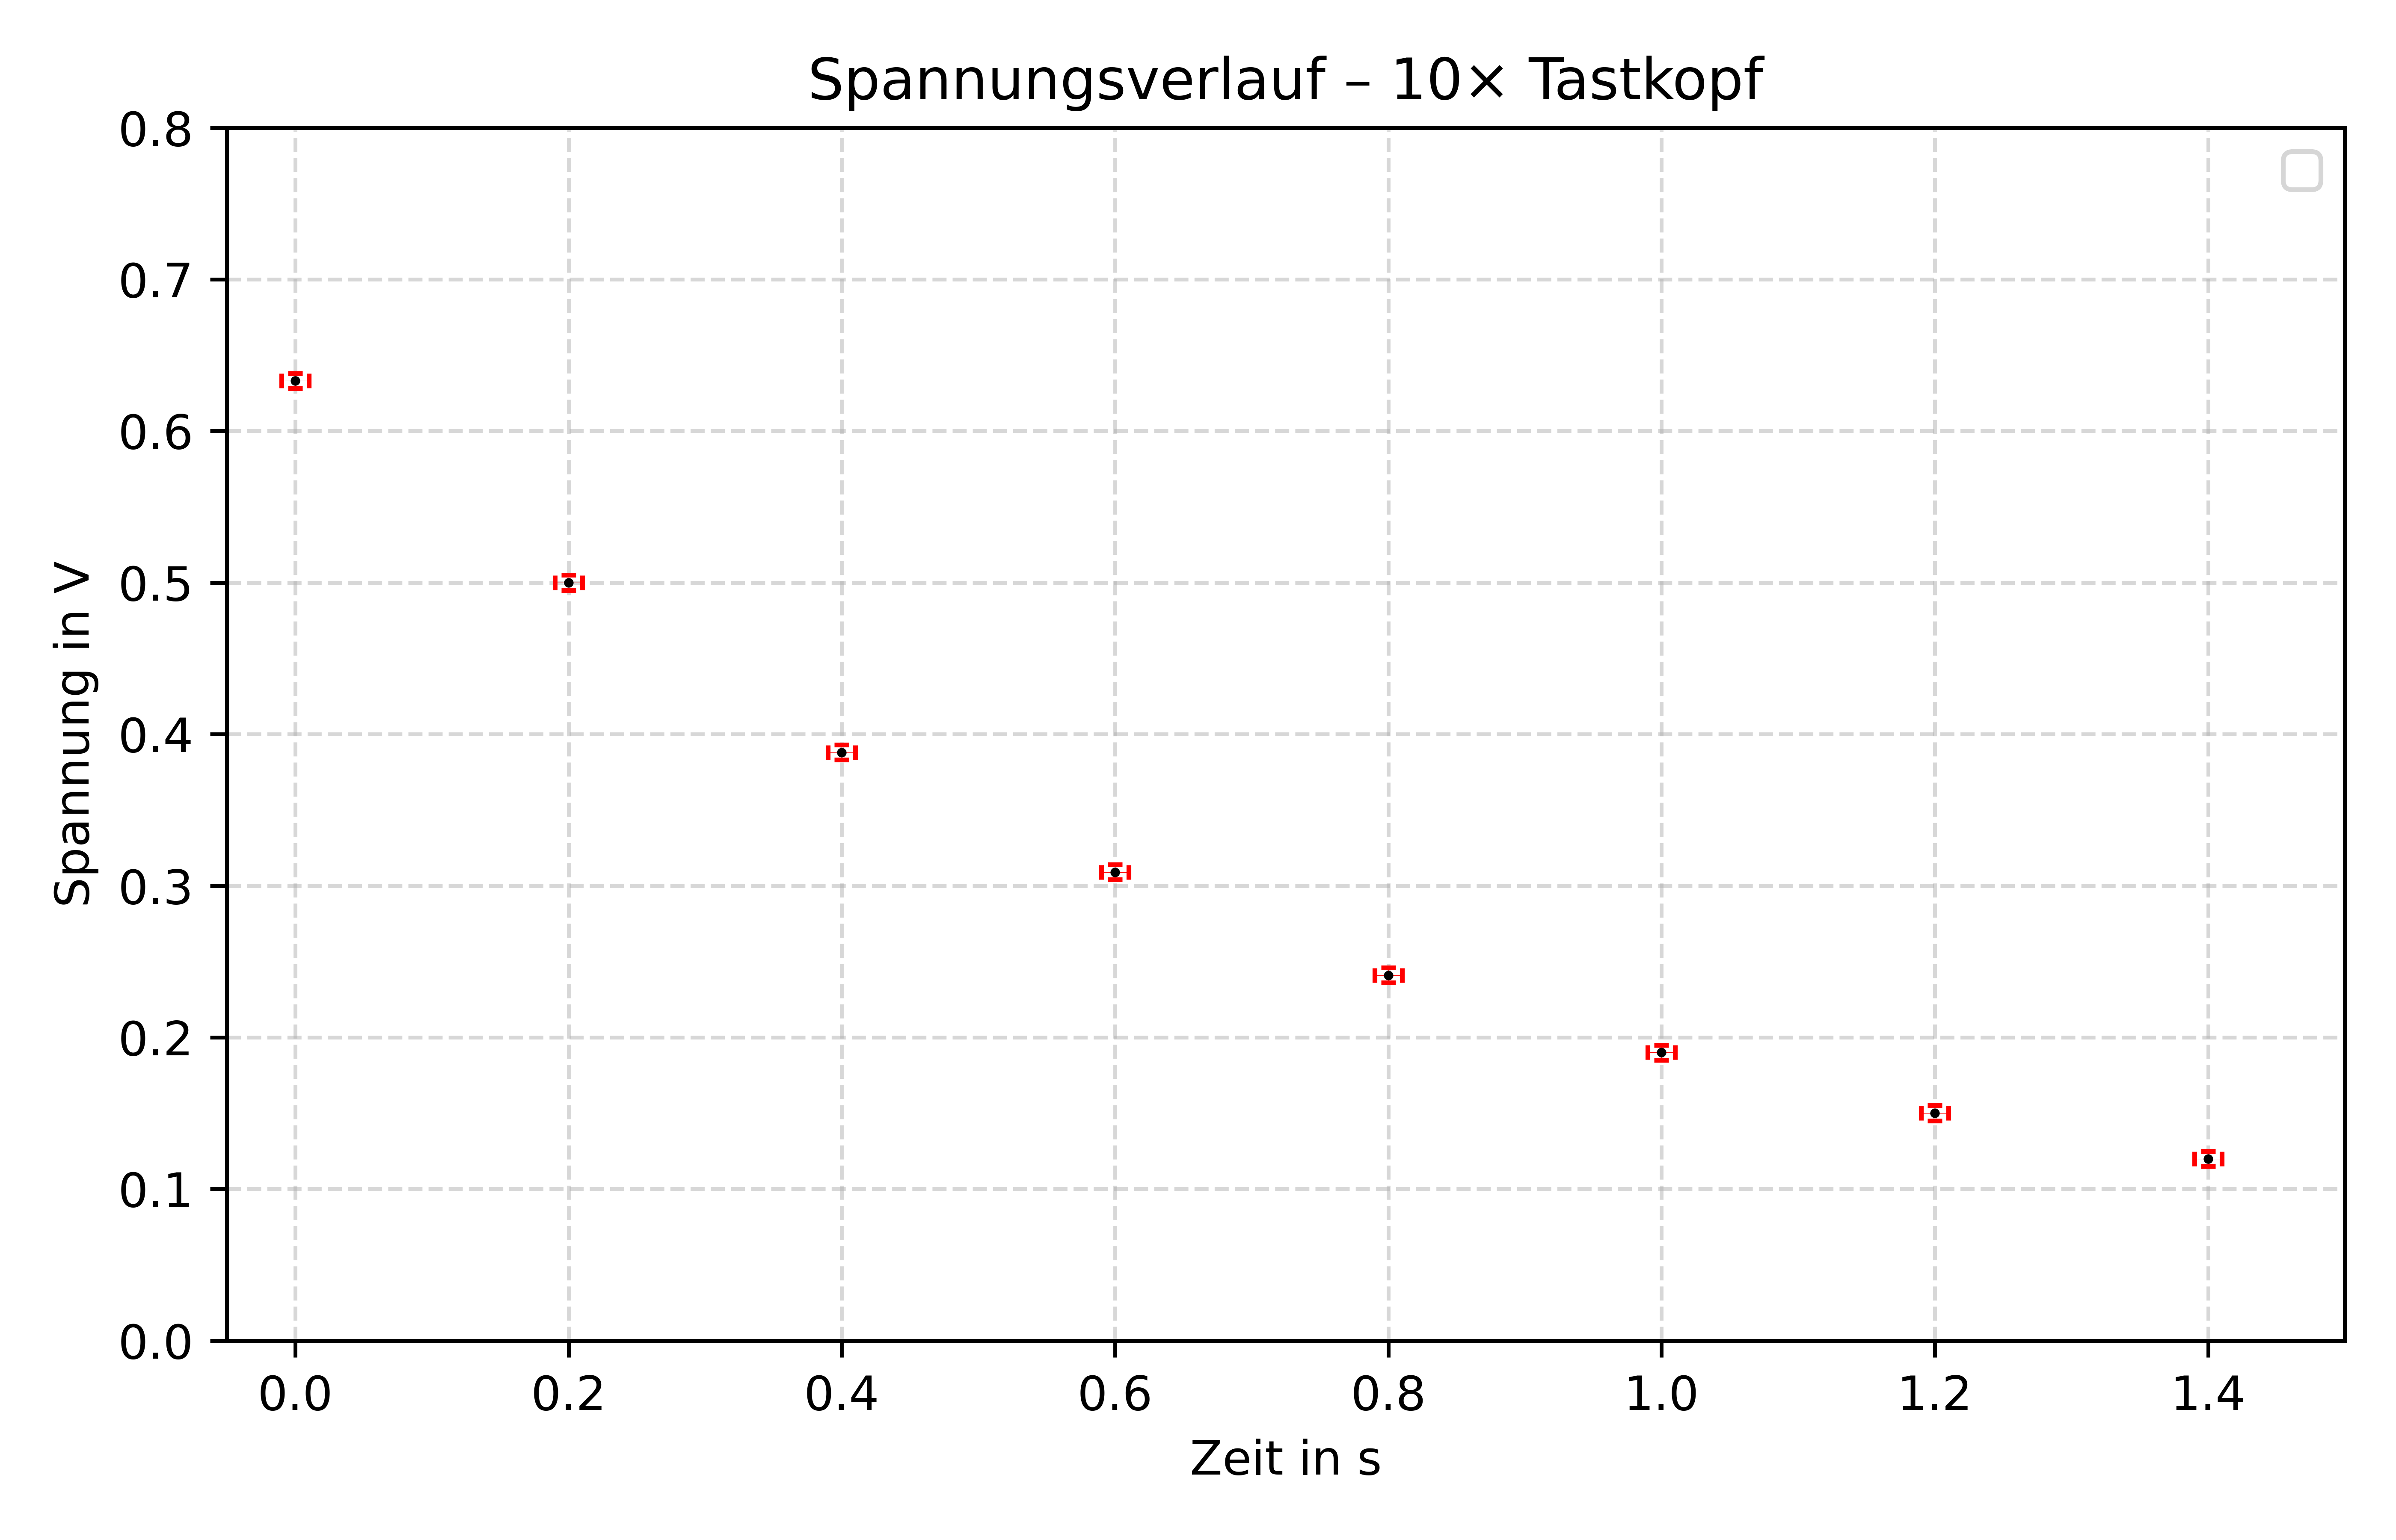
\includegraphics[width=.8\textwidth]{./Images/spannungsverlauf_10xTKRaw.png}
    \caption{Spannungsverlauf 10$\times$ Tastkopf}
    \label{fig:10xTKDiag}
\end{figure}
\newpage
\noindent
\subsection{Bestimmung der Relaxiationszeit aus den experimentellen Daten}
Um die Daten besser analysieren zu können, tragen wir im folgenden $\ln(U / \si{V})$ gegen die Zeit auf.
Für den Fehler $\Delta \ln(U/V)$ gilt:
\begin{equation}
    \begin{split}
        \Delta \ln(U/V) &= \frac{\partial}{\partial U} ln(U/V) \cdot \Delta U \\
                        &= \frac{\Delta U}{U}
    \end{split}
\end{equation}
Dieser wird also insbesondere für kleine Spannungen besonders groß.
Plottet man die Werte und Fehlerbalken mithilfe eines Python Scripts und trägt zudem die Ausgleichsgeraden durch die maximalen und minimalen Werte ein, 
erhält man folgende Diagramme:
\begin{figure}[H]
    \centering
    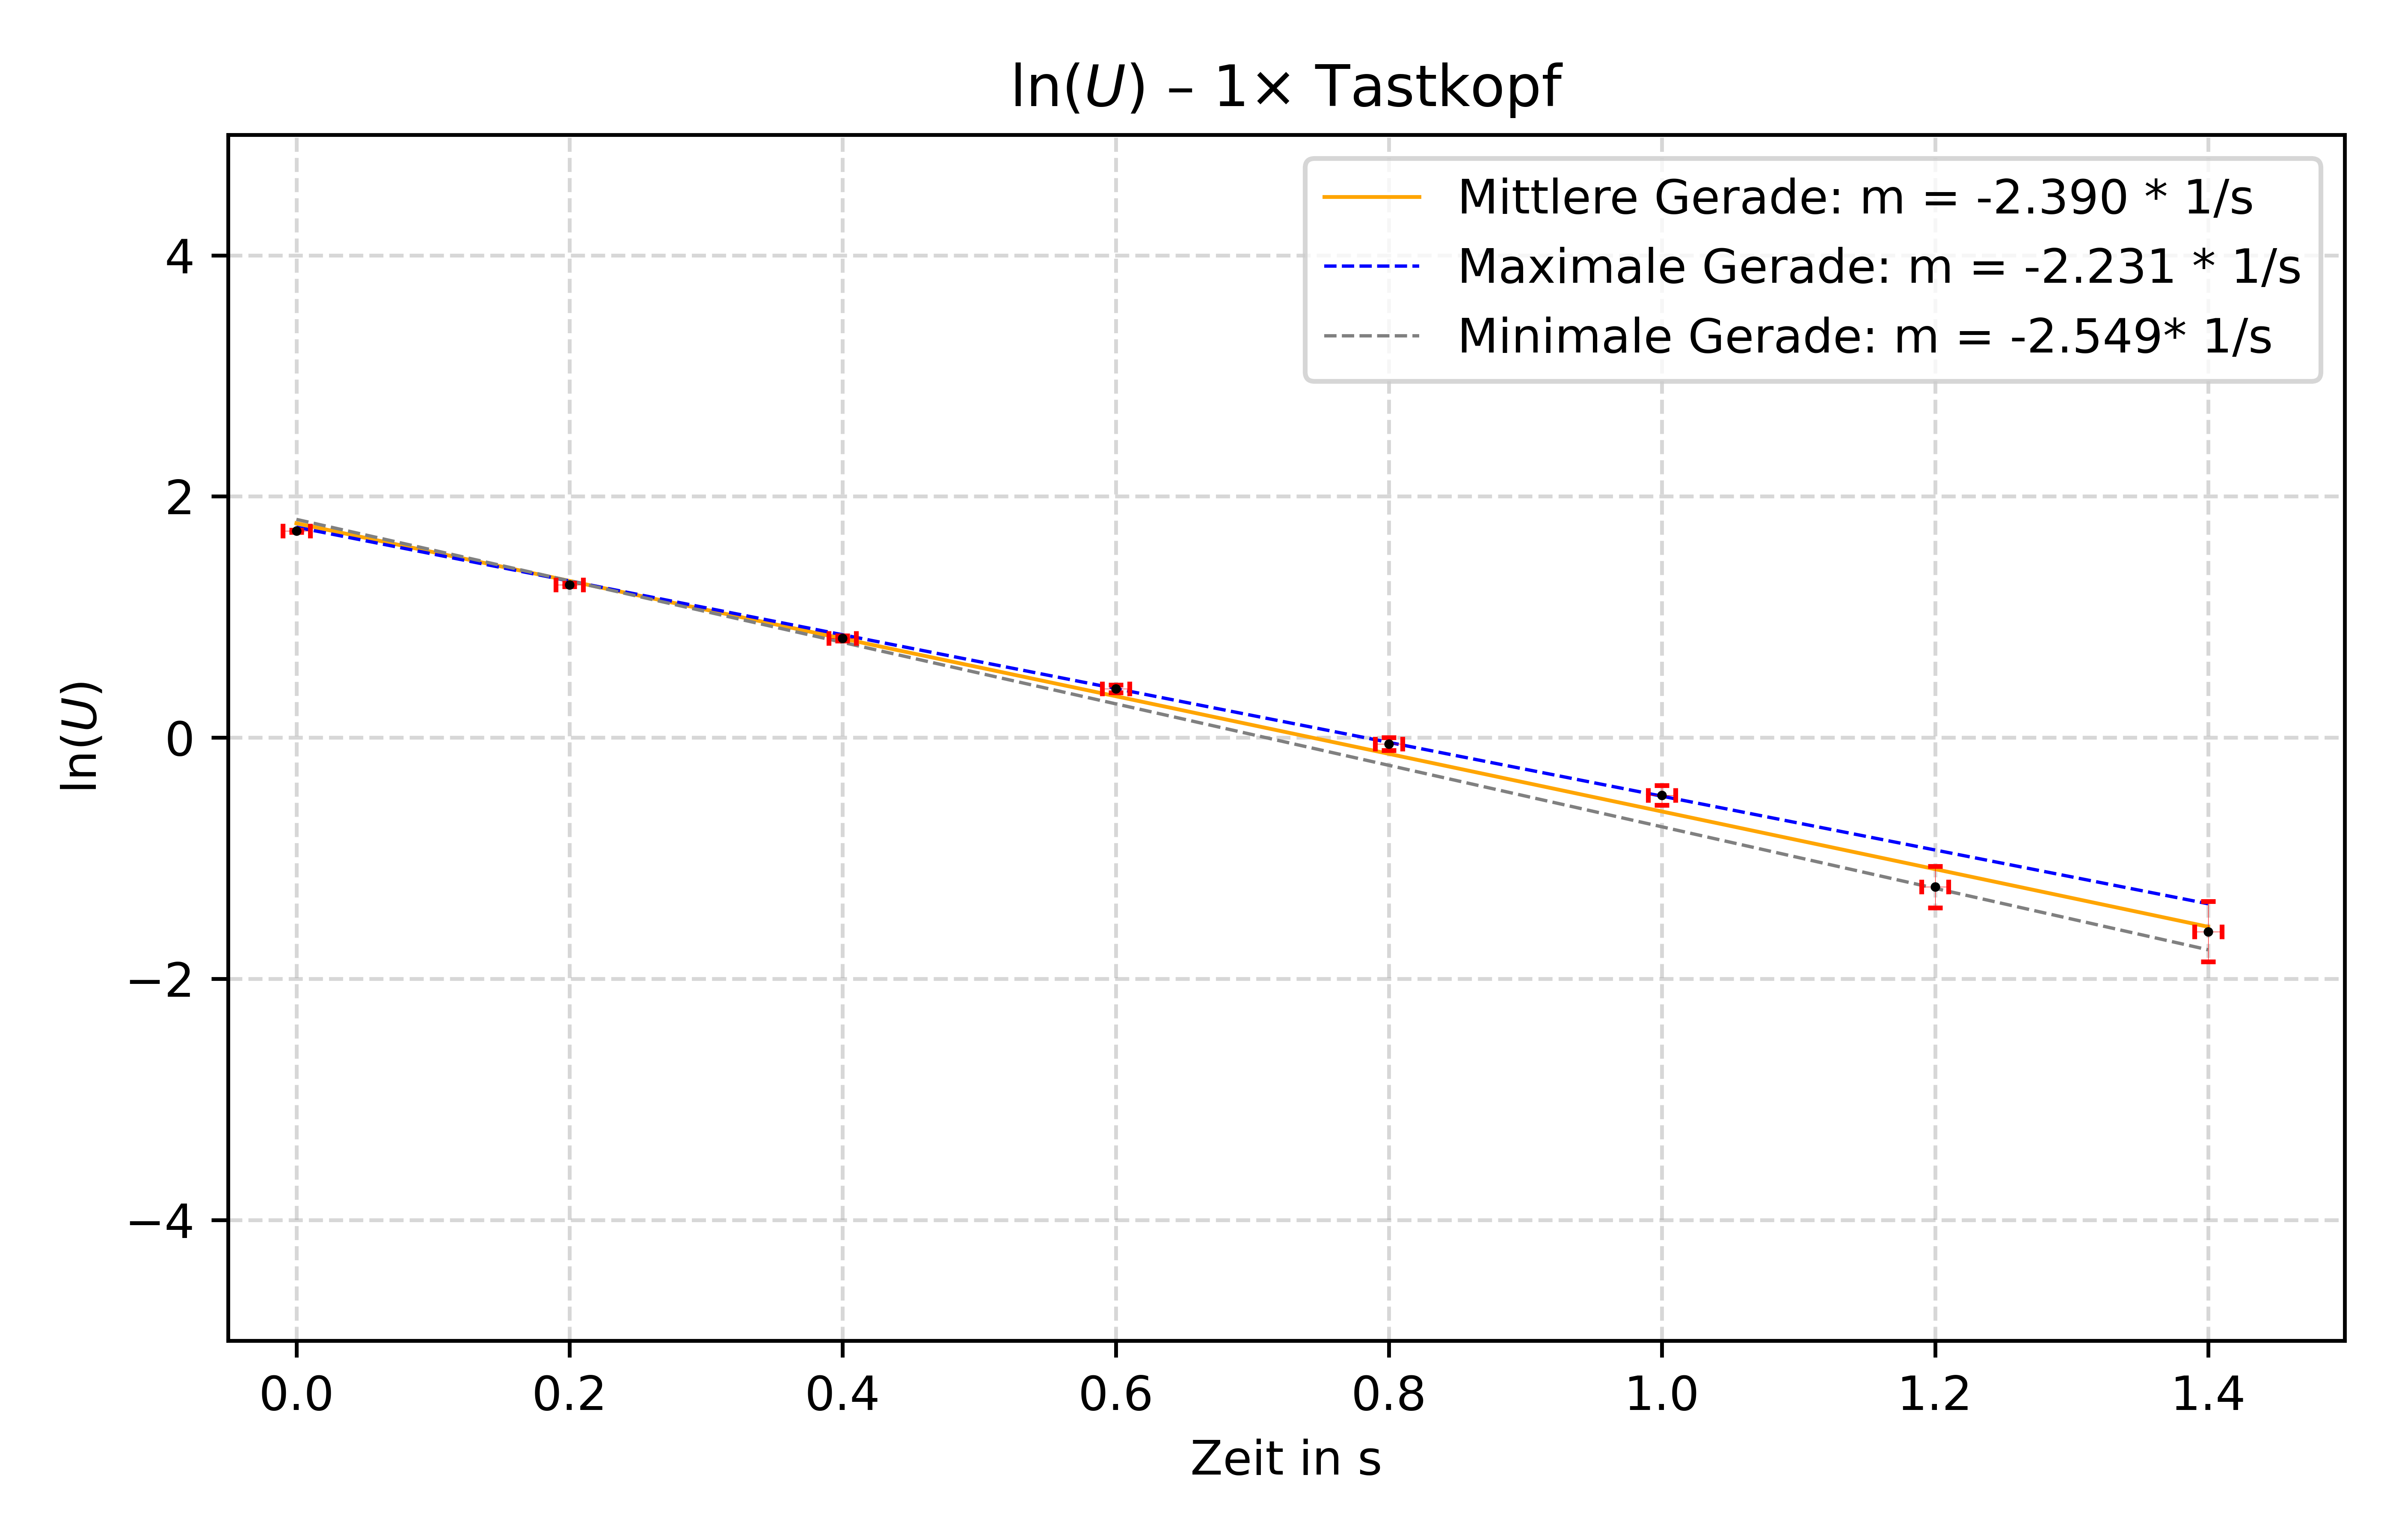
\includegraphics[width=1\textwidth]{./Images/spannungsverlauf_1xTKLog.png}
    \caption{Logarithmus der Spannung für den 1x Tastkopf}
    \label{fig:1xTKDiagLog}
\end{figure}
\begin{figure}[H]
    \centering
    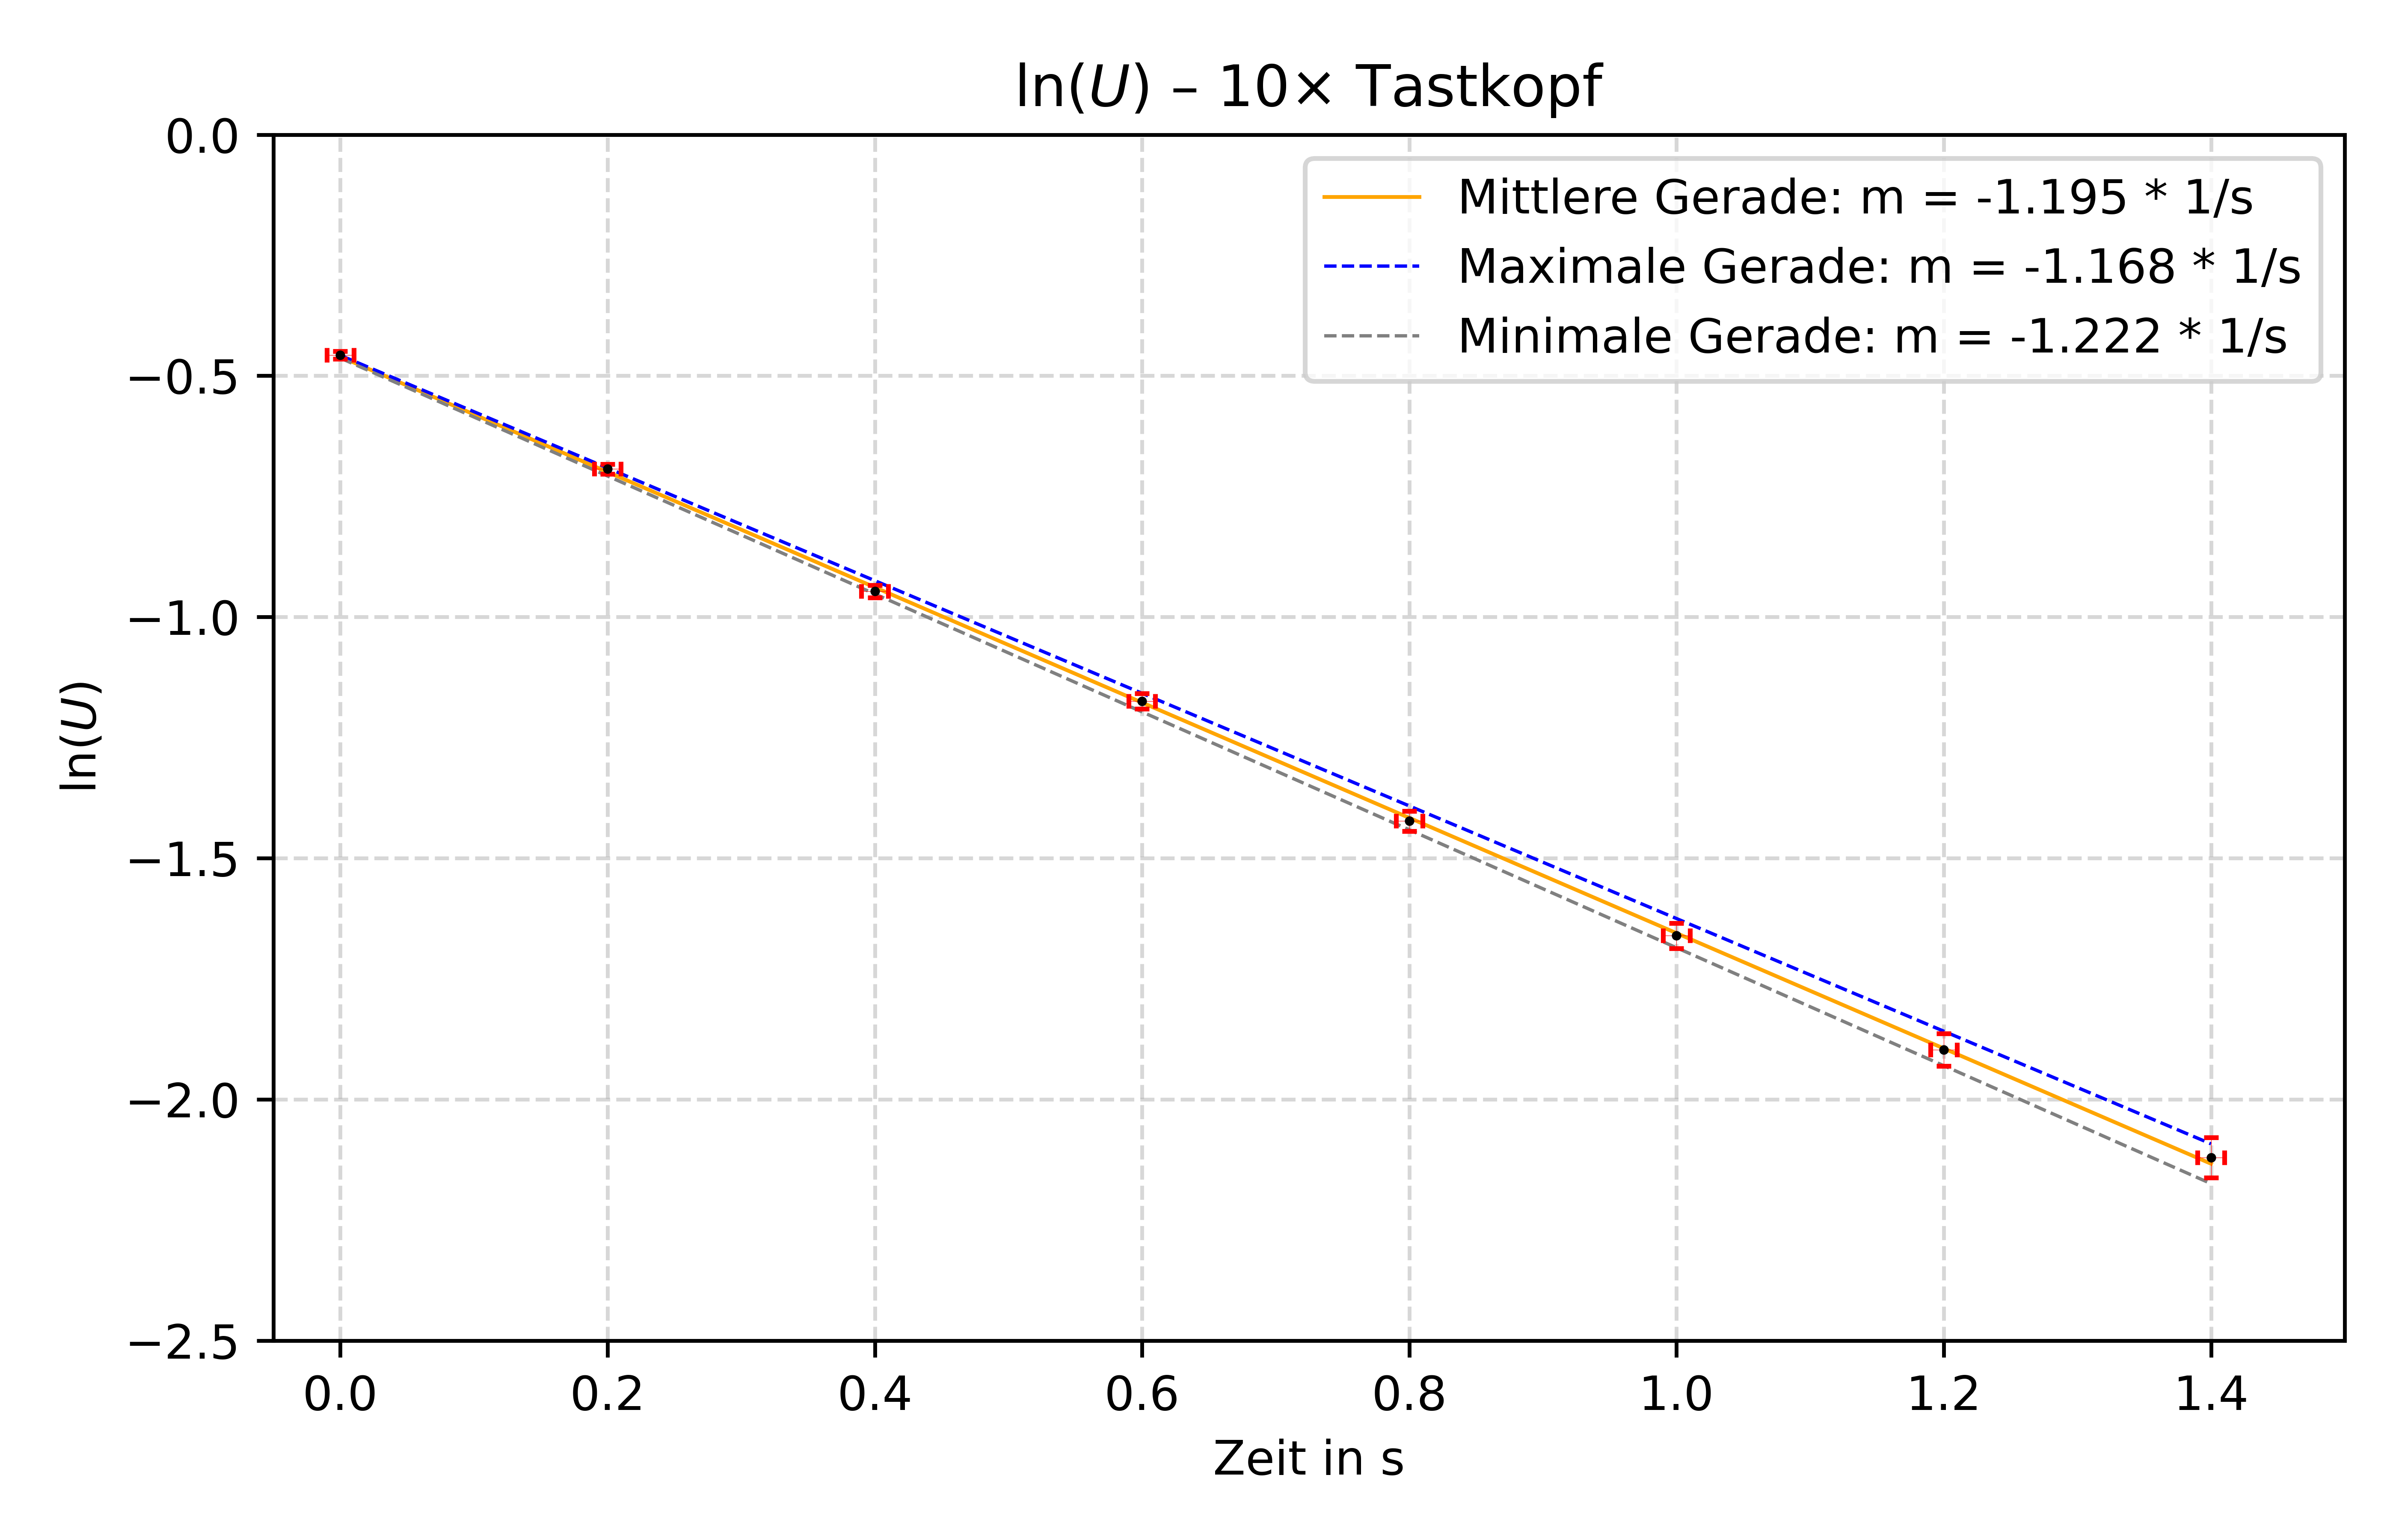
\includegraphics[width=1\textwidth]{./Images/spannungsverlauf_10xTKLog.png}
    \caption{Logarithmus der Spannung für den 10x Tastkopf}
    \label{fig:10xTKDiagLog}
\end{figure}
\noindent
Die Steigungen ist also für den 1$\times$ Tastkopf:
\begin{equation}
    m_1 = -(2.39 \pm 0.16) \frac{1}{\si{s}}
\end{equation}
Und für den 1$\times$ Tastkopf:
\begin{equation}
    m_{10} = -(1.19 \pm 0.03) \frac{1}{\si{s}}
\end{equation}
Durch die Logarithmisierung folgt folgender Zusammenhang aus dem bekannten Spannungsverlauf eines Kondensators:
\begin{equation}
    \begin{split}
        U(t) &= U_0 \cdot \exp(- \frac{t}{\tau}) \\
        \Leftrightarrow \ln(U/\si{V}) &= \ln(U_0/\si{V}) - \frac{t}{\tau} \\
                                &= \ln(U_0/\si{V}) + m \cdot t \\
        \Leftrightarrow \tau &= - \frac{1}{m}
    \end{split}
\end{equation}
Damit ist $\tau$ unabhängig von $U_0$, weshalb nicht berücksichtigt werden muss, dass durch den 10$\times$ Tastkopf $U_0$ gezehntelt wird. 
Dies hat also ausschließlich Auswirkungen auf den Ordinatenabschnitt des Diagrams. \\
Für die Unsicherheit von $\tau$ gilt:
\begin{equation}
    \begin{split}
        \Delta \tau &= \frac{\partial \tau}{\partial m} \cdot \Delta m \\
                    &= \frac{\Delta m}{m^2}
    \end{split}
\end{equation}
Somit folgt:
\begin{equation}
    \begin{split}
        \bar{\tau_1} &= 0.418 \si{s} \\
        \bar{\tau_{10}} &= 0.840 \si{s} \\
        \Delta \tau_1 &= 0.029 \si{s} \\
        \Delta \tau_{10} &= 0.022
    \end{split}
\end{equation}
Womit folgende Abklingzeiten experimentell bestimmt wurden:
\begin{equation}
    \begin{split}        
        \boxed{\tau_1 = 0.418 \pm 0.029 \si{s}} \\
        \boxed{\tau_{10} = 0.840 \pm 0.022 \si{s}}
    \end{split}
    \label{eq:experimentelleRelaxiationszeiten}
\end{equation}
\subsection{Theoretischer Wert für die Relaxiationszeit}
Der theoretisch bestimmte Wert für $\tau$ liegt bei:
\begin{equation}
    \begin{split}
        \bar{\tau}_{\mathrm{theo}}  &= RC \\
                                    &= 1.00\si{M\Omega} \cdot 1.00\si{\mu F} \\
                                    &= 1.00s
    \end{split}
\end{equation}
Für die Unsicherheit des Theoriewerts gilt mit $\Delta C = 0.1 \si{\mu F}$ und $\Delta R = 0.01 \si{M \Omega}$:
\begin{equation}
    \begin{split}
        \Delta \tau_{\mathrm{\mathrm{theo}}}    &= \sqrt{\left(\frac{\partial \tau_{\mathrm{theo}}}{\partial R} \cdot \Delta R\right)^2 + \left(\frac{\partial \tau_{\mathrm{theo}}}{\partial C} \cdot \Delta C\right)^2} \\
                                                &= \sqrt{(C \cdot \Delta R)^2 + (R \cdot \Delta C)^2} \\
                                                &\approx 0.11 \si{s}
    \end{split}
\end{equation}
Damit liegt $\tau_{\mathrm{theor}}$ bei:
\begin{equation}
    \tau_{\mathrm{theor}} =  (1.00 \pm 0.11)s   
\end{equation} 
Es ist erkennbar, dass keiner der beiden gemessenen Werte im Rahmen der Messunsicherheit mit dem Theoriewert übereinstimmt. Dies 
liegt an der Eingangskopplung. Insbesondere im Fall mit Tastkopfeinstellung $1\times$ ist der Effekt besonders signifikant. 
Dies liegt daran, dass der Innenwiderstand der Messvorrichtung parallel zum Entladewiderstand geschalten ist (Siehe Abbildung \ref{fig:Eingangskopplung}), 
was zu einem insgesamt geringeren effektiven Widerstand führt, über welchen der Kondensator entladen wird. 
In der $1\times$ Einstellung ist dies besonders signifikant, da hier der parallele Innenwiderstand bei 
gerade einmal $1 \si{M \Omega}$ liegt. Um die Abschwächung auf $\frac{1}{10}$ zu erreichen, ist im $10\times$ Modus 
ein $9\si{M \Omega}$ Widerstand in Reihe zum Innenwiderstand des Oszilloskop geschalten. Der gesamte parallele innenwiderstand 
liegt also bei insgesamt $10 \si{M \Omega}$, wodurch der effektive Widerstand, der durch die Parallelschaltung entsteht
nicht ganz so stark (aber dennoch signifikant) vom äußeren Widerstand abweicht.
Daher ist der Effekt hier weniger eindeutig erkennbar.
\begin{figure}[H]
    \centering
    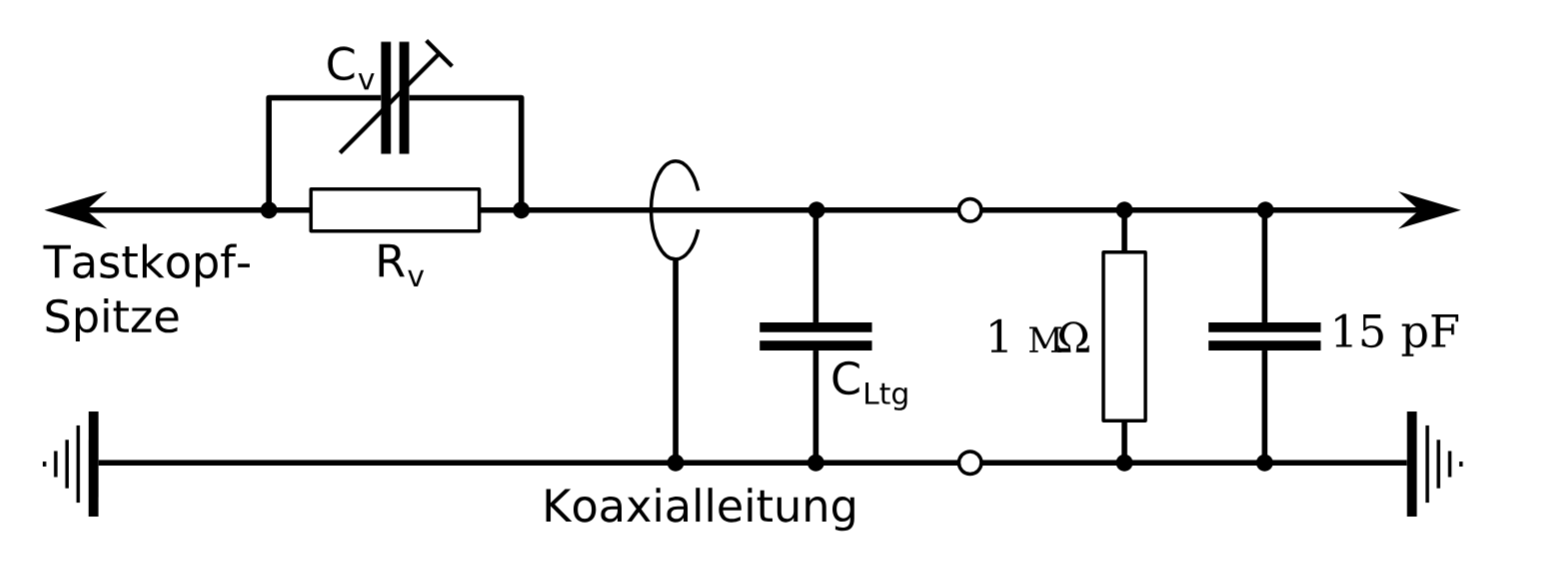
\includegraphics[width=.8\textwidth]{./Images/Eingangskopplung.png}
    \caption{Schaltbild der Eingangskopplung mit Tastkopf}
    \label{fig:Eingangskopplung}
\end{figure}
\noindent
\subsubsection{Effektivwiderstand durch Parallelschaltung mit den Innenwiderständen}
Berücksichtigt man die Innenwiderstände erhält man folgendermaßen den Effektivwiderstand:
\begin{equation}
    R_{\mathrm{eff}} = \left(\frac{1}{R} + \frac{1}{R_{\mathrm{innen}}}\right)^{-1}
\end{equation}
Wenn man davon ausgeht, dass der Effektivwiderstand wieder eine Toleranz von $1\%$ hat, erhält man mit $R_{\mathrm{innen, 1}} = 1 \si{M \Omega}$
und $R_{\mathrm{innen, 10}} = R_{\mathrm{innen, 1}} + R_{\mathrm{Tastkopf}} = 10 \si{M \Omega}$:
\begin{equation}
    \begin{split}
        R_{\mathrm{eff, 1}} &= (0.500 \pm 0.005) \si{M \Omega} \\
        R_{\mathrm{eff, 10}} &= (0.910 \pm 0.010) \si{M \Omega}
    \end{split}
\end{equation}
\subsubsection{Effektive Relaxiationszeit unter Berücksichtigung der Innenwiderstände}
Aus den Effektivwiderständen folgt äquivalent zur vorherigen Berechnung:
\begin{equation}
    \begin{split}
        \boxed{\tau_{\mathrm{theo, eff, 1}}  =  (0.50 \pm 0.06)s} \\
        \boxed{\tau_{\mathrm{theo, eff, 10}} = (0.91 \pm 0.10) s}
    \end{split}
\end{equation}
Diese Werte Stimmen im Rahmen der Messunsicherheit mit den experimentellen Messwerten überein. (\ref{eq:experimentelleRelaxiationszeiten})
\newpage
\chapter{Anhang}
\section{Python Scripts}
Die Python Scripts, die zum Plotten der Grafiken verwendet wurden, wurden mit Unterstützung von KI erstellt und dann nach den eigenen Bedürfnissen weiter
bearbeitet.
\definecolor{codegreen}{rgb}{0,0.6,0}
\definecolor{codegray}{rgb}{0.5,0.5,0.5}
\definecolor{codepurple}{rgb}{0.58,0,0.82}
\definecolor{backcolour}{rgb}{0.95,0.95,0.92}

\lstdefinestyle{python}{
    backgroundcolor=\color{backcolour},   
    commentstyle=\color{codegreen},
    keywordstyle=\color{magenta},
    numberstyle=\tiny\color{codegray},
    stringstyle=\color{codepurple},
    basicstyle=\ttfamily\footnotesize,
    breakatwhitespace=false,         
    breaklines=true,                 
    captionpos=b,                    
    keepspaces=true,                 
    numbers=left,                    
    numbersep=5pt,                  
    showspaces=false,                
    showstringspaces=false,
    showtabs=false,                  
    tabsize=2
}
\subsection{TV V:}
\subsubsection{Plot der Rohwerte}
\begin{scriptsize}
\lstset{style=python}
\begin{lstlisting}[language=python]
import matplotlib.pyplot as plt
import numpy as np

# Daten aus der Tabelle
# zeit     = [0.000, 0.200, 0.400, 0.600, 0.800, 1.000, 1.200, 1.400]
# spannung = [5.55,  3.55,  2.28,  1.50,  0.95,  0.62,  0.29,  0.20]
zeit     = [0.000, 0.200, 0.400, 0.600, 0.800, 1.000, 1.200, 1.400, 1.600]
spannung = [0.633, 0.500,  0.388,  0.309,  0.241,  0.190,  0.150,  0.120,  0.093]


# Plot
fig, ax = plt.subplots(figsize=(7, 4.5))

ax.errorbar(zeit, spannung, xerr=0.01, yerr=0.005, fmt='o', ms = '1', mec = 'black',  
            ecolor='red', elinewidth=.1, capsize=1.5,)

ax.set_xlabel("Zeit in s")
ax.set_ylabel("Spannung in V")
ax.set_title("Spannungsverlauf - 10x Tastkopf")
ax.legend()
ax.grid(True, linestyle="--", alpha=0.5)
ax.set_xlim(-0.05, 1.5)
ax.set_ylim(0, 0.8)
# plt.show()

plt.tight_layout()
plt.savefig("./01_OSZ/Images/spannungsverlauf_10xTKRaw.png", dpi=800)
\end{lstlisting}
\end{scriptsize}
\newpage
\subsubsection{Plot der logarithmisierten Werte mit Ausgleichsgeraden}
\begin{scriptsize}
\lstset{style=python}
\begin{lstlisting}[language=python]
import matplotlib.pyplot as plt
import numpy as np

zeit     = [0.000, 0.200, 0.400, 0.600, 0.800, 1.000, 1.200, 1.400]
spannung = [5.55,  3.55,  2.28,  1.50,  0.95,  0.62,  0.29,  0.20]
# zeit     = [0.000, 0.200, 0.400, 0.600, 0.800, 1.000, 1.200, 1.400, 1.600]
# spannung = [0.633, 0.500, 0.388, 0.309, 0.241, 0.190, 0.150, 0.120, 0.093]
y_err = abs(0.05 / np.array(spannung))
spannung = np.log(spannung)
coeffsMid = np.polyfit(zeit, spannung, 1)
coeffsMin = np.polyfit(zeit, spannung - y_err, 1)
coeffsMax = np.polyfit(zeit, spannung + y_err, 1)

t_fit = np.linspace(0, 1.4, 300)
lnU_fit_mid = coeffsMid[1] + coeffsMid[0]*t_fit
lnU_fit_min = coeffsMin[1] + coeffsMin[0]*t_fit
lnU_fit_max = coeffsMax[1] + coeffsMax[0]*t_fit

fig, ax = plt.subplots(figsize=(7, 4.5))

ax.plot(t_fit, lnU_fit_mid, color="orange", linewidth=.8,
        label=f"Mittlere Gerade: m = {coeffsMid[0]:.3f} 1/s")
ax.plot(t_fit, lnU_fit_max, color="blue", linewidth=.7,
        label=f"Maximale Gerade: m = {coeffsMax[0]:.3f} 1/s", linestyle="--")
ax.plot(t_fit, lnU_fit_min, color="grey", linewidth=.7,
        label=f"Minimale Gerade: m = {coeffsMin[0]:.3f} 1/s", linestyle="--")

ax.errorbar(zeit, spannung, xerr=0.01, yerr=y_err,
            fmt='o', ms='1', mec='black',
            ecolor='red', elinewidth=.1, capsize=1.5)

ax.set_xlabel("Zeit in s")
ax.set_ylabel(r"$\ln(U)$")
ax.set_title(r"$\ln(U)$ -- 1x Tastkopf")
ax.legend()
ax.grid(True, linestyle="--", alpha=0.5)
ax.set_xlim(-0.05, 1.5)
ax.set_ylim(-5, 5)

plt.tight_layout()
plt.savefig("./01_OSZ/Images/spannungsverlauf_1xTKLog.png", dpi=800)
\end{lstlisting}
\end{scriptsize}

\end{document}
